\documentclass[tikz,border=2pt]{standalone}
\usepackage{tikz}
\usepackage{amsmath,amssymb}
\usepackage{mathptmx}

\definecolor{barpurple}{RGB}{175, 0, 200}
\definecolor{barcyan}{RGB}{176, 224, 230}
\definecolor{gridgray}{RGB}{215, 215, 215}

\begin{document}
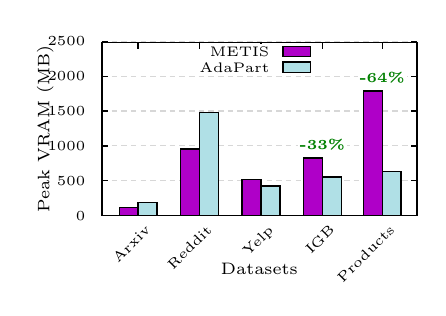
\begin{tikzpicture}

    % Plot dimensions
    \def\pw{4.0}
    \def\ph{2.2}

    % Y-axis scale: 0 to 2500 MB -> height 2.2cm (scale = 0.00088 cm/MB)
    \def\yscale{0.00088}

    % Horizontal grid lines (dashed) and Y-ticks
    \foreach \y/\lbl in {0/0, 500/500, 1000/1000, 1500/1500, 2000/2000, 2500/2500} {
        \def\yp{\y * \yscale}
        % Dashed grid line inside plot
        \ifnum\y>0
            \draw[gridgray, line width=0.4pt, dash pattern=on 2pt off 1.5pt] (0, \yp) -- (\pw, \yp);
        \fi
        % Inward ticks (gnuplot style)
        \draw[black, line width=0.5pt] (0, \yp) -- (0.08, \yp);
        \draw[black, line width=0.5pt] (\pw, \yp) -- (\pw - 0.08, \yp);
        % Left tick label with comfortable spacing
        \node[left=2.5pt, font=\fontsize{5.5}{6.5}\selectfont] at (0, \yp) {\lbl};
    }

    % Y-axis label with ample clearance
    \node[rotate=90, font=\fontsize{6.5}{7.5}\selectfont, text=black] at (-0.72, \ph/2) {Peak VRAM (MB)};

    % 5 Datasets positions
    \def\bw{0.24}

    % 1. Arxiv: 114.8 vs 185.4
    \def\xone{0.46}
    \draw[fill=barpurple, draw=black, line width=0.5pt] (\xone - \bw, 0) rectangle (\xone, 114.8 * \yscale);
    \draw[fill=barcyan, draw=black, line width=0.5pt] (\xone, 0) rectangle (\xone + \bw, 185.4 * \yscale);

    % 2. Reddit: 956.4 vs 1478.2
    \def\xtwo{1.24}
    \draw[fill=barpurple, draw=black, line width=0.5pt] (\xtwo - \bw, 0) rectangle (\xtwo, 956.4 * \yscale);
    \draw[fill=barcyan, draw=black, line width=0.5pt] (\xtwo, 0) rectangle (\xtwo + \bw, 1478.2 * \yscale);

    % 3. Yelp: 517.9 vs 426.8
    \def\xthree{2.02}
    \draw[fill=barpurple, draw=black, line width=0.5pt] (\xthree - \bw, 0) rectangle (\xthree, 517.9 * \yscale);
    \draw[fill=barcyan, draw=black, line width=0.5pt] (\xthree, 0) rectangle (\xthree + \bw, 426.8 * \yscale);

    % 4. IGB: 828.5 vs 552.9
    \def\xfour{2.80}
    \draw[fill=barpurple, draw=black, line width=0.5pt] (\xfour - \bw, 0) rectangle (\xfour, 828.5 * \yscale);
    \draw[fill=barcyan, draw=black, line width=0.5pt] (\xfour, 0) rectangle (\xfour + \bw, 552.9 * \yscale);
    \node[above=2pt, font=\fontsize{4.8}{5}\selectfont\bfseries, text=green!50!black, fill=white, inner sep=0.6pt] at (\xfour, 828.5 * \yscale) {-33\%};

    % 5. Products: 1788.7 vs 635.9
    \def\xfive{3.56}
    \draw[fill=barpurple, draw=black, line width=0.5pt] (\xfive - \bw, 0) rectangle (\xfive, 1788.7 * \yscale);
    \draw[fill=barcyan, draw=black, line width=0.5pt] (\xfive, 0) rectangle (\xfive + \bw, 635.9 * \yscale);
    \node[above=2pt, font=\fontsize{4.8}{5}\selectfont\bfseries, text=green!50!black, fill=white, inner sep=0.6pt] at (\xfive, 1788.7 * \yscale) {-64\%};

    % Outer bounding box (all 4 sides solid black)
    \draw[black, line width=0.6pt] (0, 0) rectangle (\pw, \ph);

    % Inward ticks on bottom and top borders for x categories
    \foreach \x/\lbl in {\xone/Arxiv, \xtwo/Reddit, \xthree/Yelp, \xfour/IGB, \xfive/Products} {
        \draw[black, line width=0.5pt] (\x, 0) -- (\x, 0.08);
        \draw[black, line width=0.5pt] (\x, \ph) -- (\x, \ph - 0.08);
        % Rotated label at 45 degrees
        \node[anchor=north east, rotate=45, font=\fontsize{5.5}{6.5}\selectfont, inner sep=1pt] at (\x + 0.08, -0.05) {\lbl};
    }

    % X-axis label
    \node[font=\fontsize{6.5}{7.5}\selectfont, text=black] at (\pw/2, -0.68) {Datasets};

    % Legend inside top-center (above Yelp where space is wide open)
    \begin{scope}[shift={(1.45, 2.12)}]
        \draw[fill=white, draw=none] (-0.05, -0.34) rectangle (1.25, 0.06);
        % Entry 1: METIS
        \node[left, font=\fontsize{5}{6}\selectfont] at (0.80, -0.04) {METIS};
        \draw[fill=barpurple, draw=black, line width=0.4pt] (0.85, -0.10) rectangle (1.20, 0.03);
        % Entry 2: AdaPart
        \node[left, font=\fontsize{5}{6}\selectfont] at (0.80, -0.24) {AdaPart};
        \draw[fill=barcyan, draw=black, line width=0.4pt] (0.85, -0.30) rectangle (1.20, -0.17);
    \end{scope}

\end{tikzpicture}
\end{document}

